%%%%%%%%%%%%%%%%%%%%%%%%%%%%%%%%%%%%%%%%%
% University/School Laboratory Report
% LaTeX Template
% Version 3.1 (25/3/14)
%
% This template has been downloaded from:
% http://www.LaTeXTemplates.com
%
% Original author:
% Linux and Unix Users Group at Virginia Tech Wiki 
% (https://vtluug.org/wiki/Example_LaTeX_chem_lab_report)
%
% Modified by:
% Riccardo Prinzivalle
%
% License:
% CC BY-NC-SA 3.0 (http://creativecommons.org/licenses/by-nc-sa/3.0/)
%
%%%%%%%%%%%%%%%%%%%%%%%%%%%%%%%%%%%%%%%%%

%----------------------------------------------------------------------------------------
%	PACKAGES AND DOCUMENT CONFIGURATIONS
%----------------------------------------------------------------------------------------

\documentclass{article}

\usepackage{graphicx} % Required for the inclusion of images
\usepackage[square,numbers]{natbib} % Required to change bibliography style to APA
\usepackage{amsmath} % Required for some math elements 
\usepackage[hyphens]{url} % required for url in bibliography
\usepackage{hyperref} % required for hyperlink in url
\usepackage{float} % required for positioning of table
\usepackage{pdflscape} % required for table rotation
\usepackage{array, makecell} % for multiline cells of table
\usepackage{breakurl} % for breaking url link 
%\usepackage{tabularx}
%\newcolumntype{L}{>{\raggedright\arraybackslash}X}

\setlength\parindent{0pt} % Removes all indentation from paragraphs

%\usepackage{times} % Uncomment to use the Times New Roman font

%----------------------------------------------------------------------------------------
%	DOCUMENT INFORMATION
%----------------------------------------------------------------------------------------

\title{Implementation of SED with Depthwise Separable and Dilated Convolutions \\[0.2em]\small{}Neural Networks Sapienza 2020} % Title

\author{Riccardo \textsc{Prinzivalle}} % Author name

\date{March 2021} % Date for the report

\begin{document}

\maketitle % Insert the title, author and date

%\begin{abstract}
%Some abstract text for presentation
%\end{abstract}

%----------------------------------------------------------------------------------------
%	SECTION 1
%----------------------------------------------------------------------------------------

\section{Introduction}
\label{sec:intro}

This project is a study and implementation of a polyphonic sound event detection extracted from \cite{drossos2020sound}. It is also based on the baseline reference of \cite{drossos2020sound}, which is \cite{Cakir_2017}. These two works represent the main source of this project. Here there will be presented both a replication of the paper approach together with a monophonic sound event detection, since to obtain the original dataset took some time, the author thought to start working with another dataset and then move the work to the original dataset when it would have been available. Section \ref{sec:mono} and \ref{sec:poly} are organized as follows: first an analysis of the dataset is performed to better understand it, then it is explained how the feature have been extracted and finally it is proposed a model to solve the problem. Section \ref{sec:results} regroups the results for both datasets, then it is explained a brief digression on how to train a neural network model on an AMD GPU on section \ref{sec:AMD} since the author's setup has only an AMD GPU. The work is ended by conclusions of section \ref{sec:end}.
 
%----------------------------------------------------------------------------------------
%	SECTION 2
%----------------------------------------------------------------------------------------

\section{Monophonic SED}
\label{sec:mono}

Monophonic Sound Event Detection consist of predicting a single label for an audio recording: the record will likely contain some noise but it generally contains a single and remarkable sound to be identified. In this case, it is used the \textit{UrbanSound8K} dataset \cite{Salamon:UrbanSound:ACMMM:14}.

\subsection{Data analysis}
\label{subsec:mono_analysis}

The dataset is composed by 8732 labelled small sound recordings (less than 4 seconds) from 10 classes: \textit{air\_conditioner}, \textit{car\_horn}, \textit{children\_playing}, \textit{dog\_bark}, \textit{drilling}, \textit{engine\_idling}, \textit{gun\_shot}, \textit{jackhammer}, \textit{siren}, and \textit{street\_music}. The classes are balanced except for some, it can be seen in table \ref{tab:mono_distribution}. Only 3 out of 10 classes have less than 1000 elements, so there can be some problems predicting these classes.

\begin{table}[H]
	\begin{center}
		\begin{tabular}{ |c | c | }
			\hline
			Label 				& number of elements \\ 
			\hline
			air\_conditioner 	& 1000 \\
			\hline
			car\_horn 			& 429 \\
			\hline
			children\_playing 	& 1000 \\
			\hline
			dog\_bark 			& 1000 \\
			\hline
			drilling 			& 1000 \\
			\hline
			engine\_idling 		& 1000 \\
			\hline
			gun\_shot 			& 374 \\
			\hline
			jackhammer 			& 1000 \\
			\hline
			siren 				& 929 \\
			\hline
			street\_music 		& 1000 \\
			\hline
		\end{tabular}
		\caption{Monophonic dataset label distribution}
		\label{tab:mono_distribution}
	\end{center}
\end{table}

Moreover, the recordings have different properties since they come from \url{www.freesound.org} and are taken as they are. The first difference is in the audio lengths visible in figure \ref{fig:mono_duration}: the majority of audio have a duration of about 3.5/4 seconds, but there exists also smaller recordings which are in a tiny number.

\begin{figure}[H]
	\centering
	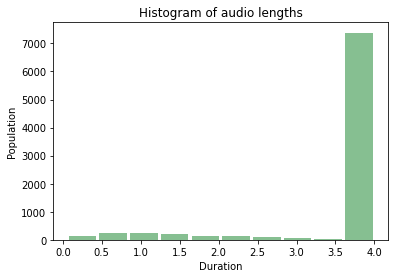
\includegraphics[width=0.8\textwidth]{./images/mono/duration.png}	
	\caption{Audio duration distribution}
	\label{fig:mono_duration}
\end{figure}

The main differences are in bit depth, from 4 to 32 bit, the majority with 16 bit; and in the sample rate, from 8 KHz to 192 KHz, with the majority with 44.1 KHz. This may be a concern since some audio have a poor quality which can translate in poorer feature w.r.t. the other tracks. All these differences will be equalized during the feature extraction phase.

\subsection{Feature Extraction}
\label{subsec:mono_feature}

This phase adopts librosa \cite{mcfee2015librosa}, which is a sound processing library for python. Its use helps to deal with different audio characteristics since by default librosa converts audio to 22 KHz sampling rate and 16 bit depth. Since the majority of audio recordings are at 44.1 KHz, it may seem that down sampling may reduce audio quality, but if we visualize the sound with a spectrogram, it will be clear that most of frequency content is distributed well below the 11 KHz (which is the maximum frequency a 22 KHz sampling rate can process), so in this case it reduces the dimension of the data without losing much information. For what concerns the bit depth, the majority of recordings are already at 16 bit, so it does not change much the data. Audio file are loaded and transformed into array series by \textit{load} function, which is also responsible of audio conversion and standardization.\newline
The reference paper \cite{drossos2020sound} uses Mel Frequency Cepstral Coefficients (MFCC) to extract features from the array sound data. MFCCs are a way of measuring the rate of information change in spectral bands and storing it in coefficients; moreover, the rate of change is modeled in a non linear way since the Mel band is logarithmic and the adoption of this band is able to capture the rate of change in a similar way to what the human hear does \cite{MFCC}. \newline
The idea is to extract the MFCC with the basic settings and change just the number of feature extracted per frame to 40 to adapt it to reference paper \cite{drossos2020sound}. The principal basic setting is using a window of 2048 bit for the Fast Fourier Transform inside the MFCC extractor, the other settings are of minor importance in this case. The correspondence between the window and a temporal interval is given by the following formula: 
 
\begin{equation} \label{eq:window_interval}
	window\_interval = \cfrac{bit\_ftt}{sampling\_rate}
\end{equation}

This means that if the sampling rate is 22 KHz and the number of bit is 2048, then the window interval is about 93 ms. The execution shows that 93 ms are too much for just 3 recordings which have a smaller duration. The result of feature extraction is a matrix of 40 features by a varying length depending on the length of the processed audio. Here a problem arises: a neural network may only process input of equal length, so the smaller recordings are padded with zeros to reach the dimension of the longer audio, which has a length of 174 frames. The data are ready to be feed as input of the neural network now.\newline
A small technical digression: since python based libraries for sound processing are easier to use but slower, the extracted features are saved in pickle file to be easily loaded without reprocessing every time the dataset \cite{pickle}.\newline
Processed data are labeled with a categorical encoding using \textit{keras utils} and \textit{sklearn preprocessing} in automatic way.

\subsection{Model formulation}
\label{subsec:mono_model}

This work presents two different model architectures for monophonic SED, both derived from \cite{drossos2020sound}: a baseline architecture, composed by convolutional and recurrent layers, and a proposed model, which is constituted by depth-wise separable convolutions followed by dilated convolutions.\newline
Each model accepts an input of the following form: the first dimension is time, so the 174 frames, then the feature dimension (40) and the channel dimension, used by the convolution, which is just one since no convolution has been applied yet.\newline
The baseline model is composed by 3 convolutional layer and 1 recurrent layer. Each convolution is followed by batch normalization, max pooling and dropout. Each convolution uses 256 channel, 5x5 kernel, unitary stride and ReLU activation function. Padding is added to preserve the input dimension (\textit{same} padding). Max pooling is performed with different kernel dimension in the layers: (1,5), (1,4) and (1,2) respectively, with same padding to maintain dimension: this strange arrangement of pooling is to obtain a unitary feature dimension at the end of the third convolutional layer and preserve unchanged the time dimension. Dropout is added to reduce overfitting and it has a rate of 0.25. Since feature dimension is reduced to a unit, the tensor is reshaped to a matrix composed by the number of frames as rows and the number of channel as columns. This tensor is the input of the recurrent layer, which is a Gated Recurrent Unit of 256 unit. The output of the GRU is the input of a dense layer with 10 outputs and softmax activation function. The role of the 3 components is the following: the convolutions acts as feature extractor from the MFCCs, the GRU are used to identify temporal pattern and the dense layer is used as classifier. The model is trained using adam as optimizer, with categorical cross-entropy as cost function and categorical accuracy as metric. Adam optimizer is used with standard parameters \cite{kingma2017adam}.\newline
\textbf{ADD MODEL IMAGE}
\newline
The proposed approach substitutes the convolutional layers with depth-wise separable convolutions and the recurrent layer with dilated convolution. Parameters are equal to the previous model, the only difference is that dilated convolution output has 3 dimension plus the batch size, so a global average pooling is used to reduce the dimension to feed the dense layer. This is a modification of the proposed approach of \cite{drossos2020sound} since the dilated convolution are designed to output a tensor which can be reshaped to a 2D output to maintain temporal frames, instead in this case it is necessary to just assign a single category to all the frames together since only one sound is contained in each audio input, so I decided to use global average pooling to connect dilated convolution and the dense layer. Initially I tried to apply a convolution with unitary kernel and (1,3) stride to reduce dimension, followed by a max pooling to connect to dense layer but it produced worse result and I adopted the global average pooling solution; in both cases of proposed approach performs very poorly compared to baseline model, as it will be seen in section \ref{sec:results}. This is due to the fact that the proposed model was developed for polyphonic SED and it is adapted to this case, probably a better formulation is possible for this specific case.\newline
\textbf{ADD MODEL IMAGE}

%----------------------------------------------------------------------------------------
%	SECTION 3
%----------------------------------------------------------------------------------------

\section{Polyphonic SED}
\label{sec:poly}

Polyphonic SED, instead, is more complicate: the idea is to have recordings with multiple overlapping sounds and to detect correctly the category of each single sound and the instants when the sound starts and ends (the maximum polyphony is 5). The dataset used is \textit{TUT-SED Synthetic 2016} \cite{Cakir_2017}, which is a synthetic dataset, while the section \ref{sec:mono} dataset is composed by recordings in real spaces and not modified in any way. Details on how the dataset has been created can be found at \url{https://webpages.tuni.fi/arg/paper/taslp2017-crnn-sed/tut-sed-synthetic-2016}.

\subsection{Data analysis}
\label{subsec:poly_analysis}

The dataset is composed by 100 long sound recordings (about some minutes) containing a mixture of different sound events. Each mixture contains multiple labels specified by onset and offset of each single sound event. Dataset contains a total of 36326 events distributed in 16 classes, the distribution can be seen in table \ref{tab:poly_distribution}.

\begin{table}[H]
	\begin{center}
		\begin{tabular}{ |c | c | }
			\hline
			Label 				& number of elements \\ 
			\hline
			footsteps 			& 8302 \\
			\hline
			horsewalk			& 6603 \\
			\hline
			bird\_singing 		& 6079 \\
			\hline
			baby\_crying 		& 3342 \\
			\hline
			dog\_barking 		& 3145 \\
			\hline
			gun\_shot 			& 1581 \\
			\hline
			crowd\_applause 	& 1400 \\
			\hline
			cat\_meowing 		& 885 \\
			\hline
			motorcycle 			& 824 \\
			\hline
			thunder 			& 774 \\
			\hline
			glass\_smash 		& 693 \\
			\hline
			crowd\_cheering 	& 613 \\
			\hline
			alarms\_and\_sirens & 571 \\
			\hline
			mixer 				& 547 \\
			\hline
			rain 				& 511 \\
			\hline
			bus 				& 456 \\
			\hline
		\end{tabular}
		\caption{Monophonic dataset label distribution}
		\label{tab:poly_distribution}
	\end{center}
\end{table}

From the table, it is easily visible that classes are not distributed equally, moreover they have different duration, for example \textit{rain} is a class with rather long duration while \textit{horsewalk} contains very small duration events. As a rule of thumb of this dataset, one can enounce that the longer the duration the smaller the number of appearances, and vice versa. An histogram of audio lengths distribution can be found in figure \ref{fig:poly_duration}; this confirms the rule of thumb.

\begin{figure}[H]
	\centering
	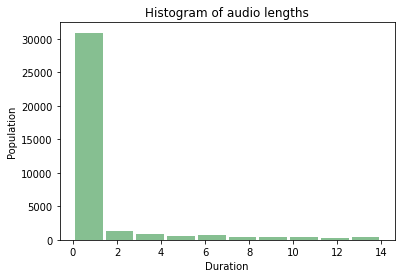
\includegraphics[width=0.9\textwidth]{./images/poly/duration.png}	
	\caption{Decision trees assembly only confusion matrix}
	\label{fig:poly_duration}
\end{figure}

Since the dataset is synthetic, audio properties are unique for all the mixtures: single channel, 32 bit depth and 44.1 KHz sampling rate.

\subsection{Feature Extraction}
\label{subsec:poly_feature}

This case will use the same technique of monophonic SED in section \ref{subsec:mono_feature}: the audio is loaded and transformed to 16 bit depth and 22 KHz sampling rate, this is done to reduce the dimensionality of processed data and speed up computation at cost of small losses of audio quality.\newline
MFCCs are extracted with different parameters in this case: the number of feature per frame is 40, with 40 mel bands, 20 ms window and 50 \% overlap. This means, using formula \ref{eq:window_interval}, that it is necessary to use 440 bit per window and 220 for the hop length since it is required a 50 \% overlap (this means that the following frame extracted starts at half of the preceding frame).\newline
Extracted data are then subdivided in sub-vectors of features composed by 1024 time frames: this is done to create an equal input for the neural network and enlarge the input data, instead of having less vectors of greater length. Moreover, this allows to standardize the input dimension in an easy way, since at most it is required to pad 1023 frames, while processing each extracted vector without subdivision would have brought bigger padding and much wasted computational power.

\subsection{Data labeling}
\label{subsec:poly_label}

Since here we are dealing with polyphonic SED, the data labeling is more complex of what it has been seen in section \ref{subsec:mono_feature}. Data are labeled manually with a one hot encode: each sub-vector is instead a matrix of 1024 time frames by 40 features, and each time frame must be labeled with 16 possible classes; a zero if the class is not present and 1 if the class is present in the chosen time frame. This method will output a 1024 time frame by 16 classes matrix which will be used as ground truth during the training. This way of labeling will eventually bring a label matrix whose composition is mainly based on zeros, which will made a hard problem but the model proposed are able to bring satisfactory results.

\subsection{Model formulation}
\label{subsec:poly_model}

This section will explain multiple model architecture introduced for poly SED: a baseline, a dilated baseline, a dessed baseline and a dessed-dilated approach (\textit{dessed stands for depth-wise separable convolution based model}). Each model has input of 1024 time frame times 40 features times 1 channel and outputs a 1024 time frame by 16 classes matrix.\newline
The baseline model is similar to the one used in section \ref{subsec:mono_model}, but the GRU is configured to give back also the time frame and not only the features. Other different parameters are the activation function of dense layer, a \textit{sigmoid}, the loss function, \textit{binary cross-entropy}, and the metric, \textit{binary accuracy}. \newline
\textbf{ADD MODEL IMAGE} \newline
The dilated baseline substitutes the recurrent neural network with a dilated convolution: the block comprehend a dilated convolution, batch normalization, max pooling and dropout; it is followed by a 1x1 convolution with (1,3) stride since the original paper \cite{drossos2020sound} uses a dilated convolution directly with stride (1,3) but the framework used in this project (keras) does not allow to specify both dilation and stride different from 1, so I though that a possible solution to overcome that could have been to use the 1x1 convolution with (1,3) stride. All other unspecified parameters are unchanged and equal to baseline model. The adoption of dilated convolutions allows to model log temporal context, reduce parameters number and eliminate the dissolving gradient for longer temporal sequences.\newline
\textbf{ADD MODEL IMAGE} \newline
The dessed baseline substitutes the convolutional layers with depth-wise separable convolutions; all other operations and parameters are equal to the baseline. This substitution allows to drastically reduce the amount of used parameters in the firsts layers.\newline
\textbf{ADD MODEL IMAGE} \newline
The combination of dessed and dilated model is what the reference paper \cite{drossos2020sound} proposes as new approach to polyphonic SED, which theoretically should decrement the total number of parameters of about 7 times and give better prediction. During the training phase I had to propose a modification of the dilated part since the 1x1 convolution block does not work well in cooperation with depth-wise separable convolution so I adopted a max pooling operation with kernel and stride of dimension (1,3) and this gives satisfying results.\newline
\textbf{ADD MODEL IMAGE} \newline

dilated convolution block (convolution, batch normalization, max pooling and dropout) is followed 



%----------------------------------------------------------------------------------------
%	SECTION 4
%----------------------------------------------------------------------------------------

\section{Experimental Results}
\label{sec:results}

\subsection{Monophonic results}
\label{subsec:mono_results}

\subsection{Polyphonic results}
\label{subsec:poly_results}

%----------------------------------------------------------------------------------------
%	SECTION 5
%----------------------------------------------------------------------------------------

\section{How to train NN on AMD GPU}
\label{sec:AMD}

%----------------------------------------------------------------------------------------
%	SECTION 6
%----------------------------------------------------------------------------------------

\section{Conclusions}
\label{sec:end}


%----------------------------------------------------------------------------------------
%	BIBLIOGRAPHY
%----------------------------------------------------------------------------------------

%\bibliographystyle{abbrv}
\bibliographystyle{unsrt}

\bibliography{bibliography}

%\nocite{*} % in case no ciattion was done or not all references has been cited 

%----------------------------------------------------------------------------------------


\end{document}